\documentclass[11pt,a4paper]{article}

\usepackage[utf8]{inputenc}
\usepackage[margin=1in]{geometry}
\usepackage{booktabs}
\usepackage{amsmath}
\usepackage{graphicx}
\usepackage{float}
\usepackage{tikz}
\usetikzlibrary{shapes,arrows,positioning}

\title{\textbf{Inter-IIT Round 2: Synthetic Dataset Generation}\\
\large A Simple Approach Using Generator Fusion}
\author{Team Solution}
\date{}

\begin{document}
\maketitle

%-------------------------------------------------------------------
\section{What We Did (Summary)}
%-------------------------------------------------------------------

\textbf{Problem:} We have 5 generators (G1-G5). Each gives us only SOME columns. We need ALL 12 columns in one dataset.

\textbf{Our Solution:} 
\begin{enumerate}
    \item Pick G3 as the ``base'' (it has the most connections to other generators)
    \item Find matching rows from other generators using shared columns
    \item Combine everything into one final dataset with 1000 rows
\end{enumerate}

\textbf{Result:} 1000 rows $\times$ 12 columns (exactly what was required)

%-------------------------------------------------------------------
\section{How We Connected the Generators}
%-------------------------------------------------------------------

Each generator shares some columns with others. We use these shared columns to find matching rows.

\begin{figure}[H]
\centering
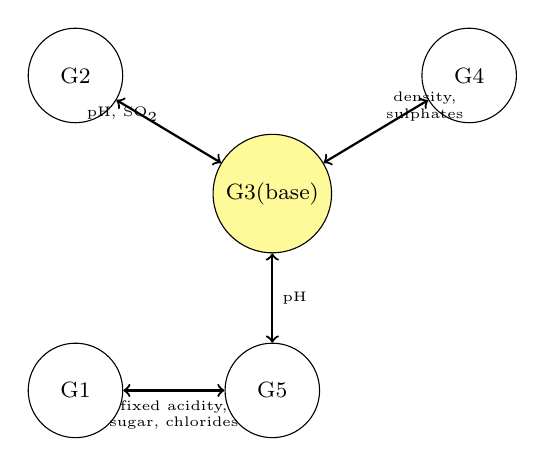
\begin{tikzpicture}[
    gen/.style={circle, draw, minimum size=1.2cm, font=\footnotesize},
    arrow/.style={<->, thick},
    label/.style={font=\tiny, align=center}
]
\node[gen, fill=yellow!40] (g3) at (0,0) {G3\\(base)};
\node[gen] (g2) at (-2.5,1.5) {G2};
\node[gen] (g4) at (2.5,1.5) {G4};
\node[gen] (g5) at (0,-2.5) {G5};
\node[gen] (g1) at (-2.5,-2.5) {G1};

\draw[arrow] (g3) -- node[label, above left] {pH, SO$_2$} (g2);
\draw[arrow] (g3) -- node[label, above right] {density,\\sulphates} (g4);
\draw[arrow] (g3) -- node[label, right] {pH} (g5);
\draw[arrow] (g5) -- node[label, below] {fixed acidity,\\sugar, chlorides} (g1);
\end{tikzpicture}
\caption{How generators are connected through shared columns}
\end{figure}

%-------------------------------------------------------------------
\section{Step-by-Step Process}
%-------------------------------------------------------------------

\subsection{Step 1: Start with G3}

We generate 1000 rows from G3. This gives us 5 columns:
\begin{center}
free SO$_2$, total SO$_2$, density, pH, sulphates
\end{center}

\subsection{Step 2: Get alcohol and quality from G4}

G3 and G4 both have ``density'' and ``sulphates''. So:
\begin{itemize}
    \item For each G3 row, find the G4 row with the closest density and sulphates
    \item Take ``alcohol'' and ``quality'' from that G4 row
\end{itemize}

\subsection{Step 3: Get fixed acidity, sugar, chlorides from G5}

G3 and G5 both have ``pH''. So:
\begin{itemize}
    \item For each G3 row, find the G5 row with the closest pH
    \item Take ``fixed acidity'', ``residual sugar'', ``chlorides'' from that G5 row
\end{itemize}

\subsection{Step 4: Get volatile acidity and citric acid from G1 and G2}

\begin{itemize}
    \item G2 shares columns with G3 $\rightarrow$ match G2 to G3
    \item G1 shares columns with G5 $\rightarrow$ match G1 to G5 (which is already matched to G3)
    \item Take volatile acidity and citric acid from both, average them
\end{itemize}

\subsection{Step 5: Final Result}

Now we have all 12 columns for each of the 1000 rows!

%-------------------------------------------------------------------
\section{Making the Data More Realistic}
%-------------------------------------------------------------------

We added some wine chemistry rules:

\textbf{Rule 1: pH depends on acidity}
\begin{itemize}
    \item More acid $\rightarrow$ lower pH
    \item We trained a small model to predict pH from acidity values
    \item Final pH = mix of predicted pH and matched pH
\end{itemize}

\textbf{Rule 2: Density depends on sugar and alcohol}
\begin{itemize}
    \item More sugar $\rightarrow$ higher density
    \item More alcohol $\rightarrow$ lower density
    \item We trained a model for this too
\end{itemize}

\textbf{Rule 3: Free SO$_2$ must be less than Total SO$_2$}
\begin{itemize}
    \item This is always true in real wine
    \item If any row violates this, we fix it
\end{itemize}

%-------------------------------------------------------------------
\section{Better Matching (Not Just 1 Neighbor)}
%-------------------------------------------------------------------

Instead of finding just 1 closest match, we find 5 and average them:

\begin{center}
\begin{tabular}{ccc}
\textbf{Simple Way} & & \textbf{Our Way (Better)} \\
Find 1 closest row & $\rightarrow$ & Find 5 closest rows \\
Take its value & $\rightarrow$ & Average their values \\
Might be bad match & $\rightarrow$ & Smoother, more reliable \\
\end{tabular}
\end{center}

%-------------------------------------------------------------------
\section{Where Each Column Comes From}
%-------------------------------------------------------------------

\begin{table}[H]
\centering
\begin{tabular}{@{}ll@{}}
\toprule
\textbf{Column} & \textbf{Source} \\
\midrule
free sulfur dioxide & G3 (base) \\
total sulfur dioxide & G3 (base) \\
density & G3 + chemistry model \\
pH & G3 + chemistry model \\
sulphates & G3 (base) \\
alcohol & G4 (matched) \\
quality & G4 (matched) \\
fixed acidity & G5 (matched) \\
residual sugar & G5 (matched) \\
chlorides & G5 (matched) \\
volatile acidity & G1 + G2 (averaged) \\
citric acid & G1 + G2 (averaged) \\
\bottomrule
\end{tabular}
\caption{Final column sources}
\end{table}

%-------------------------------------------------------------------
\section{Validation (Did It Work?)}
%-------------------------------------------------------------------

\begin{table}[H]
\centering
\begin{tabular}{@{}lcc@{}}
\toprule
\textbf{Check} & \textbf{Expected} & \textbf{Result} \\
\midrule
Number of rows & 1000 & 1000 \checkmark \\
Number of columns & 12 & 12 \checkmark \\
Missing values & 0 & 0 \checkmark \\
Free SO$_2$ $\leq$ Total SO$_2$ & Always & Always \checkmark \\
pH in normal range & Yes & Yes \checkmark \\
\bottomrule
\end{tabular}
\caption{All checks passed}
\end{table}

%-------------------------------------------------------------------
\section{How to Run It}
%-------------------------------------------------------------------

\begin{enumerate}
    \item Open Kaggle, create notebook with GPU
    \item Add the dataset ``round-2-inter-iit''
    \item Run our notebook: \texttt{physics\_informed\_notebook.ipynb}
    \item Get output: \texttt{physics\_informed\_dataset.csv}
    \item Done! Takes about 1 minute.
\end{enumerate}

%-------------------------------------------------------------------
\section{Files We Submit}
%-------------------------------------------------------------------

\begin{table}[H]
\centering
\begin{tabular}{@{}ll@{}}
\toprule
\textbf{File} & \textbf{What It Is} \\
\midrule
\texttt{physics\_informed\_dataset.csv} & The final 1000 $\times$ 12 dataset \\
\texttt{physics\_informed\_notebook.ipynb} & Code to generate it \\
\texttt{report.pdf} & This document \\
\bottomrule
\end{tabular}
\end{table}

\vspace{1cm}
\hrule
\vspace{0.3cm}
\textit{Inter-IIT Data + Generative AI Challenge - Round 2}

\end{document}
